\documentclass{article} % This command is used to set the type of document you are working on such as an article, book, or presenation

\usepackage{geometry} % This package allows the editing of the page layout
\usepackage{amsmath}  % This package allows the use of a large range of mathematical formula, commands, and symbols
\usepackage{graphicx}  % This package allows the importing of images
\usepackage{soul}
\usepackage{amsfonts, amsmath}
\usepackage{dirtytalk}
\usepackage{tabto}
\usepackage{xcolor,colortbl, amssymb}
\usepackage{forest, tikz}
\usepackage{fontawesome}
\usepackage[ruled, lined, linesnumbered, commentsnumbered, longend]{algorithm2e}

% https://www.messletters.com/en/big-text/

\newcommand{\question}[2][]{\begin{flushleft}
        \textbf{Problem #1}: \textit{#2}

\end{flushleft}}

\definecolor{Green}{rgb}{0, 1, 0}
\definecolor{Pink}{rgb}{1, .753, .796}

\newcommand{\sol}{\textbf{Solution}:} %Use if you want a boldface solution line
%\newcommand\tab[1][0.4cm]{\hspace*{#1}}
\newcommand{\maketitletwo}[2][]{\begin{center}
        \Large{\textbf{Homework #1}
            
            CMPSC 465} % Name of course here
        \vspace{5pt}
        
        \normalsize{Kinner Parikh  % Your name here
        
        \today}        % Change to due date if preferred
        \vspace{40pt}


        \newpage
        
\end{center}}
\begin{document}
    \maketitletwo[1]  % Optional argument is assignment number
    %Keep a blank space between maketitletwo and \question[1]

    \question[1]{}
    \begin{center}
        
        I did not work in a group
    
        I did not consult without anyone my group member
    
        I did not consult any non-class materials
    \end{center}
    
    \newpage

    \question[2]{DFS Basics}

    a) $A,\ B,\ D,\ E,\ G,\ F,\ C,\ H,\ I$

    \vspace{5pt}

    
    b) $A(1, 12), B(2, 11), D(3, 6), E(4, 5), G(7, 10), F(8, 9), C(13, 18), H(14, 17), I(15, 16)$
    
    \vspace{5pt}
    
    c) Tree Edges: \hspace{16pt}\{$(A, B), (B, D), (D, E), (B, G), (G, F), (C, H), (H, I)$\}
    
    \hspace{12pt}Back Edges: \hspace{14pt}\{$(E, D)$\}
    
    \hspace{12pt}Forward Edges: \{$(A, E), (C, I)$\}
    
    \hspace{12pt}Cross Edges: \hspace{12pt}\{$(G, D)$\}

    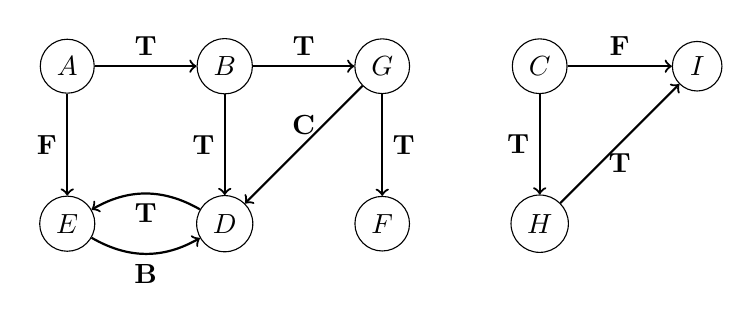
\begin{tikzpicture}[scale=2,auto=center]

        \node[circle, draw] (a) at (1, 2) {$A$};
        \node[circle, draw] (b) at (2, 2) {$B$};
        \node[circle, draw] (c) at (4, 2) {$C$};
        \node[circle, draw] (d) at (2, 1) {$D$};
        \node[circle, draw] (e) at (1, 1) {$E$};
        \node[circle, draw] (f) at (3, 1) {$F$};
        \node[circle, draw] (g) at (3, 2) {$G$};
        \node[circle, draw] (h) at (4, 1) {$H$};
        \node[circle, draw] (i) at (5, 2) {$I$};

        \draw[->, thick] (a) tonode[above]{\textbf{T}} (b);
        \draw[->, thick] (a) tonode[left]{\textbf{F}} (e);
        \draw[->, thick] (b) tonode[left]{\textbf{T}} (d);
        \draw[->, thick] (b) tonode[above]{\textbf{T}} (g);
        \draw[->, thick] (c) tonode[left]{\textbf{T}} (h);
        \draw[->, thick] (c) tonode[above]{\textbf{F}} (i);
        \draw[->, thick] (d) to[bend right]node[below]{\textbf{T}} (e);
        \draw[->, thick] (e) to[bend right]node[below]{\textbf{B}} (d);
        \draw[->, thick] (g) to node[above]{\textbf{C}} (d);
        \draw[->, thick] (g) to node[right]{\textbf{T}} (f);
        \draw[->, thick] (h) to node[right, below]{\textbf{T}} (i);
        % \draw[->, thick] (c) to[bend right] (e);
        % \draw[->, thick] (d) to[bend left] (f);
        % \draw[->, thick] (f) to (g);
        % \draw[->, thick] (f) to[bend right] (h);
    \end{tikzpicture}

    \newpage

    \question[3]{Pre and Post Processing}

    a)
    
    Claim: if $\{u,v\}$ is an edge in an undirected graph, and during depth-first search 
    
    $\texttt{post}(u)<\texttt{post}(v)$, then $v$ is an ancestor of $u$ in the DFS tree.

    \vspace{5pt}
    
    Proof:

    We know there is an edge between $u$ and $v$. Given a DFS tree, there are two cases to consider 
    
    given that $\texttt{post}(u)<\texttt{post}(v)$. Furthermore, we must follow the property that for node $n$, 

    $\texttt{pre}(n)<\texttt{post}(n)$. 

    \vspace{7pt}

    Case 1: $\texttt{pre}(v)<\texttt{pre}(u)<\underline{\texttt{post}(u)<\texttt{post}(v)}$

    \vspace{2pt}

    This represents a forward (tree) edge in the graph. According to the DFS algorithm, once $v$ has
    
    been visited, we must explore the neighbors of $v$, and after all of $v$'s ancestors have been explored, 
    
    will we assign $v$'s post number. Thus, we can confidently say that $v$ is an ancestor of $u$. 

    \vspace{7pt}

    Case 2: $\texttt{pre}(u)<\underline{\texttt{post}(u)<\texttt{pre}(v)<\texttt{post}(v)}$
    
    \vspace{2pt}

    According to the DFS algorithm, we know that once $u$ has been visited, all of its neighbors and
    
    descendants must be visited before looking at $v$. This means that there exists no edge $\{u, v\}$ \faBolt

    \vspace{2pt}

    Therefore, we can say that if $\texttt{post}(u)<\texttt{post}(v)$, then $v$ is an ancestor of $u$. $\square$

    \vspace{10pt}

    b)

    We can preprocess the graph by running a DFS algorithm on the graph and assigning pre and 
    
    post numbers to each of the nodes and storing them in a data structure that has constant lookup
    
    time. In this case, the data structure can be a hash map where the key is the value of the node
    
    and the value is the pre and post numbers stored in an array. Then, when we want to find if $u$

    is an ancestor of $v$, we can simply refer to the data structure and see if $\texttt{post}(v) < \texttt{post}(u)$, and 
    
    if so, based on the proof above, we can say that $u$ is an ancestor of $v$.

    

    % \begin{algorithm}
    %     \caption{Preprocessing a graph to find all node's pre and post numbers}
% 
    %     \SetKwFunction{findMajorityElement}{findMajorityElement}
    %     \SetKwInOut{KwIn}{Input}
    %     \SetKwInOut{KwOut}{Output}
% 
    %     \KwIn{$T = (V,E)$ (in adjacency list format)}
    %     \KwOut{HashMap of all nodes (key: node value, value: array [pre(node), post(node)])}
% 
    %     $map \leftarrow \text{HashMap(value, int[2])}$
    %     
% 
    % \end{algorithm}


    \newpage

    \question[4]{Linearization Basics}

    a) (pre, post)
    
    \vspace{5pt}

    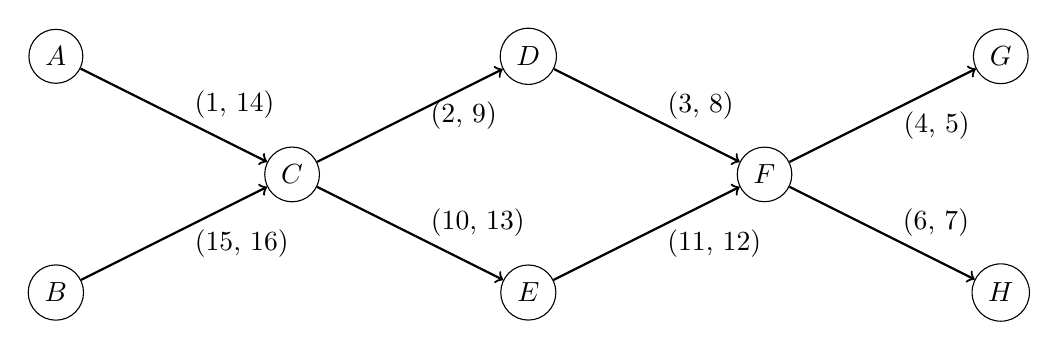
\begin{tikzpicture}[scale=1.5,auto=center]

        \node[circle, draw] (a) at (1, 4-1) {$A$};
        \node[circle, draw] (b) at (1, 2-1) {$B$};
        \node[circle, draw] (c) at (3, 3-1) {$C$};
        \node[circle, draw] (d) at (5, 4-1) {$D$};
        \node[circle, draw] (e) at (5, 2-1) {$E$};
        \node[circle, draw] (f) at (7, 3-1) {$F$};
        \node[circle, draw] (g) at (9, 4-1) {$G$};
        \node[circle, draw] (h) at (9, 2-1) {$H$};

        \path[->,draw,thick]
        (a) edge node[label = right:\text{(1, 14)}, above]{} (c)
        (b) edge node[label = right:\text{(15, 16)}, below]{} (c)
        (c) edge node[label = right:\text{(2, 9)}]{} (d)
        (c) edge node[label = right:\text{(10, 13)}, above]{} (e)
        (d) edge node[label = right:\text{(3, 8)}, above]{} (f)
        (e) edge node[label = right:\text{(11, 12)}, below]{} (f)
        (f) edge node[label = right:\text{(4, 5)}, below]{} (g)
        (f) edge node[label = right:\text{(6, 7)}, above]{} (h)
        ;
        
    \end{tikzpicture}

    $A$: (1, 14)
    $B$: (15, 16)
    $C$: (2, 9)
    $D$: (10, 13)
    $E$: (3, 8)
    $F$: (11, 12)
    $G$: (4, 5)
    $H$: (6, 7)

    \vspace{5pt}

    b) Source Nodes: $A, B$

    \hspace{10pt} Sink Nodes: $G, H$

    \vspace{5pt}

    c)

    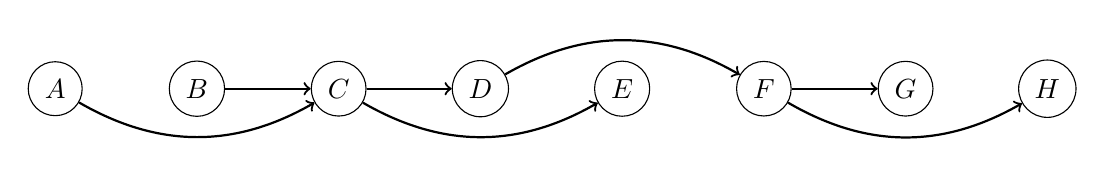
\begin{tikzpicture}[scale=0.9,auto=center]
        \node[circle, draw] (a) at (0, 0) {$A$};
        \node[circle, draw] (b) at (2, 0) {$B$};
        \node[circle, draw] (c) at (4, 0) {$C$};
        \node[circle, draw] (d) at (6, 0) {$D$};
        \node[circle, draw] (e) at (8, 0) {$E$};
        \node[circle, draw] (f) at (10, 0) {$F$};
        \node[circle, draw] (g) at (12, 0) {$G$};
        \node[circle, draw] (h) at (14, 0) {$H$};


        \draw[->, thick] (a) to[bend right] (c);
        \draw[->, thick] (b) to (c);
        \draw[->, thick] (c) to (d);
        \draw[->, thick] (c) to[bend right] (e);
        \draw[->, thick] (d) to[bend left] (f);
        \draw[->, thick] (f) to (g);
        \draw[->, thick] (f) to[bend right] (h);
        
    \end{tikzpicture}

    \vspace{5pt}

    d) This graph will have 8 total linearizations because at node $C$ and node $F$, we can go in two 
    
    \hspace{12pt}different directions. Furthermore, we could either start from $A$ or $B$, so that gives us 2 more 
    
    \hspace{12pt}options. Thus, $2 \cdot 2 \cdot 2 = 8$.
\end{document}
